% !TeX root = ../Formelsammlung.tex
\section{Grundlagen}
\subsection{Koordinatiensysteme}
\begin{equation}
\begin{pmatrix} x \\ y \\ z\end{pmatrix} = 
\begin{pmatrix}r \sin\vartheta \cos\varphi \\ r \sin\vartheta \sin\varphi \\ r \cos\vartheta \end{pmatrix} =
\begin{pmatrix}\rho \cos\varphi \\ \rho \sin\varphi \\ z \end{pmatrix}
\end{equation}
\begin{equation}
\begin{pmatrix} r \\ \varphi \\ \vartheta \end{pmatrix} =
\begin{pmatrix} \sqrt{x^2 + y^2 + z^2}  \\ \arctan\left(y/x\right) \\ \arctan\left(z/r\right) \end{pmatrix}
,\quad
\begin{pmatrix} \rho \\ \varphi \\ z \end{pmatrix} =
\begin{pmatrix} \sqrt{x^2 + y^2} \\ \arctan\left(y/x\right) \\ z \end{pmatrix}
\end{equation}

\subsection{Das Vektorprodukt}
\begin{center}
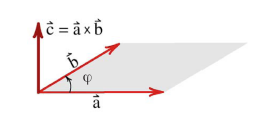
\includegraphics[scale=0.4]{./images/VectorProduct.png}
\end{center}
\begin{equation}
\vec{c} = \vec{a} \times \vec{b} \quad\Rightarrow\quad \vec{\abs{c}} = \vec{\abs{a}}\vec{\abs{b}}\sin\varphi
\end{equation}

\subsection{Ableitungen von Vektoren}
\begin{equation}
\diff{}{t}\left(c \cdot \vec{a}\right) =  \left( \diff{c}{t} \cdot \vec{a} \right) + \left( c \cdot \diff{\vec{a}}{t} \right) 
\end{equation}
\begin{equation}
\diff{}{t}\left(\vec{a} \cdot \vec{b}\right) =  \left( \diff{\vec{a}}{t} \cdot \vec{b} \right) + \left( \vec{a} \cdot \diff{\vec{b}}{t} \right) 
\end{equation}
\begin{equation}
\diff{}{t}\left(\vec{a} \times \vec{b}\right) =  \left( \diff{\vec{a}}{t} \times \vec{b} \right) + \left( \vec{a} \times \diff{\vec{b}}{t} \right) 
\end{equation}

\subsection{Lokales Systeme}
\subsubsection{Kugelkoordinaten}
Die lokalen Einheitsvektoren sind $\e{r}, \e{\vartheta}, \e{\varphi} $ wobei gilt:
\begin{itemize}
\item $\e{r}$ ist radial.
\item $\e{\vartheta}$ zeigt in die Richtung in welche sich der Punkt bewegt wenn $\vartheta$ zunimmt.
\item $\e{\varphi}$ zeigt in die Richtung in welche sich der Punkt bewegt wenn $\varphi$ zunimmt.
\end{itemize}
\begin{center}
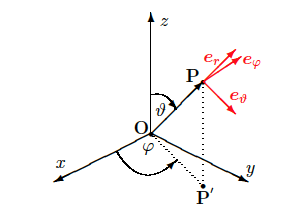
\includegraphics[scale=0.5]{./images/Kugeleinheitsvektoren.png}
\end{center}
\begin{equation}
\begin{pmatrix}
\e{r} \\ \e{\vartheta} \\ \e{\varphi}
\end{pmatrix} =
\begin{pmatrix}
\sin\vartheta\cos\varphi 	& \sin\vartheta\sin\varphi 	& \cos\vartheta \\
\cos\vartheta\cos\varphi 	& \cos\vartheta\sin\varphi 	& -\sin\vartheta \\
-\sin\varphi				 	& \cos\varphi			 	& 0
\end{pmatrix}
\begin{pmatrix}
\e{x} \\
\e{y} \\
\e{z}
\end{pmatrix}
\end{equation}